\begin{figure}[htbp]
  \centering
  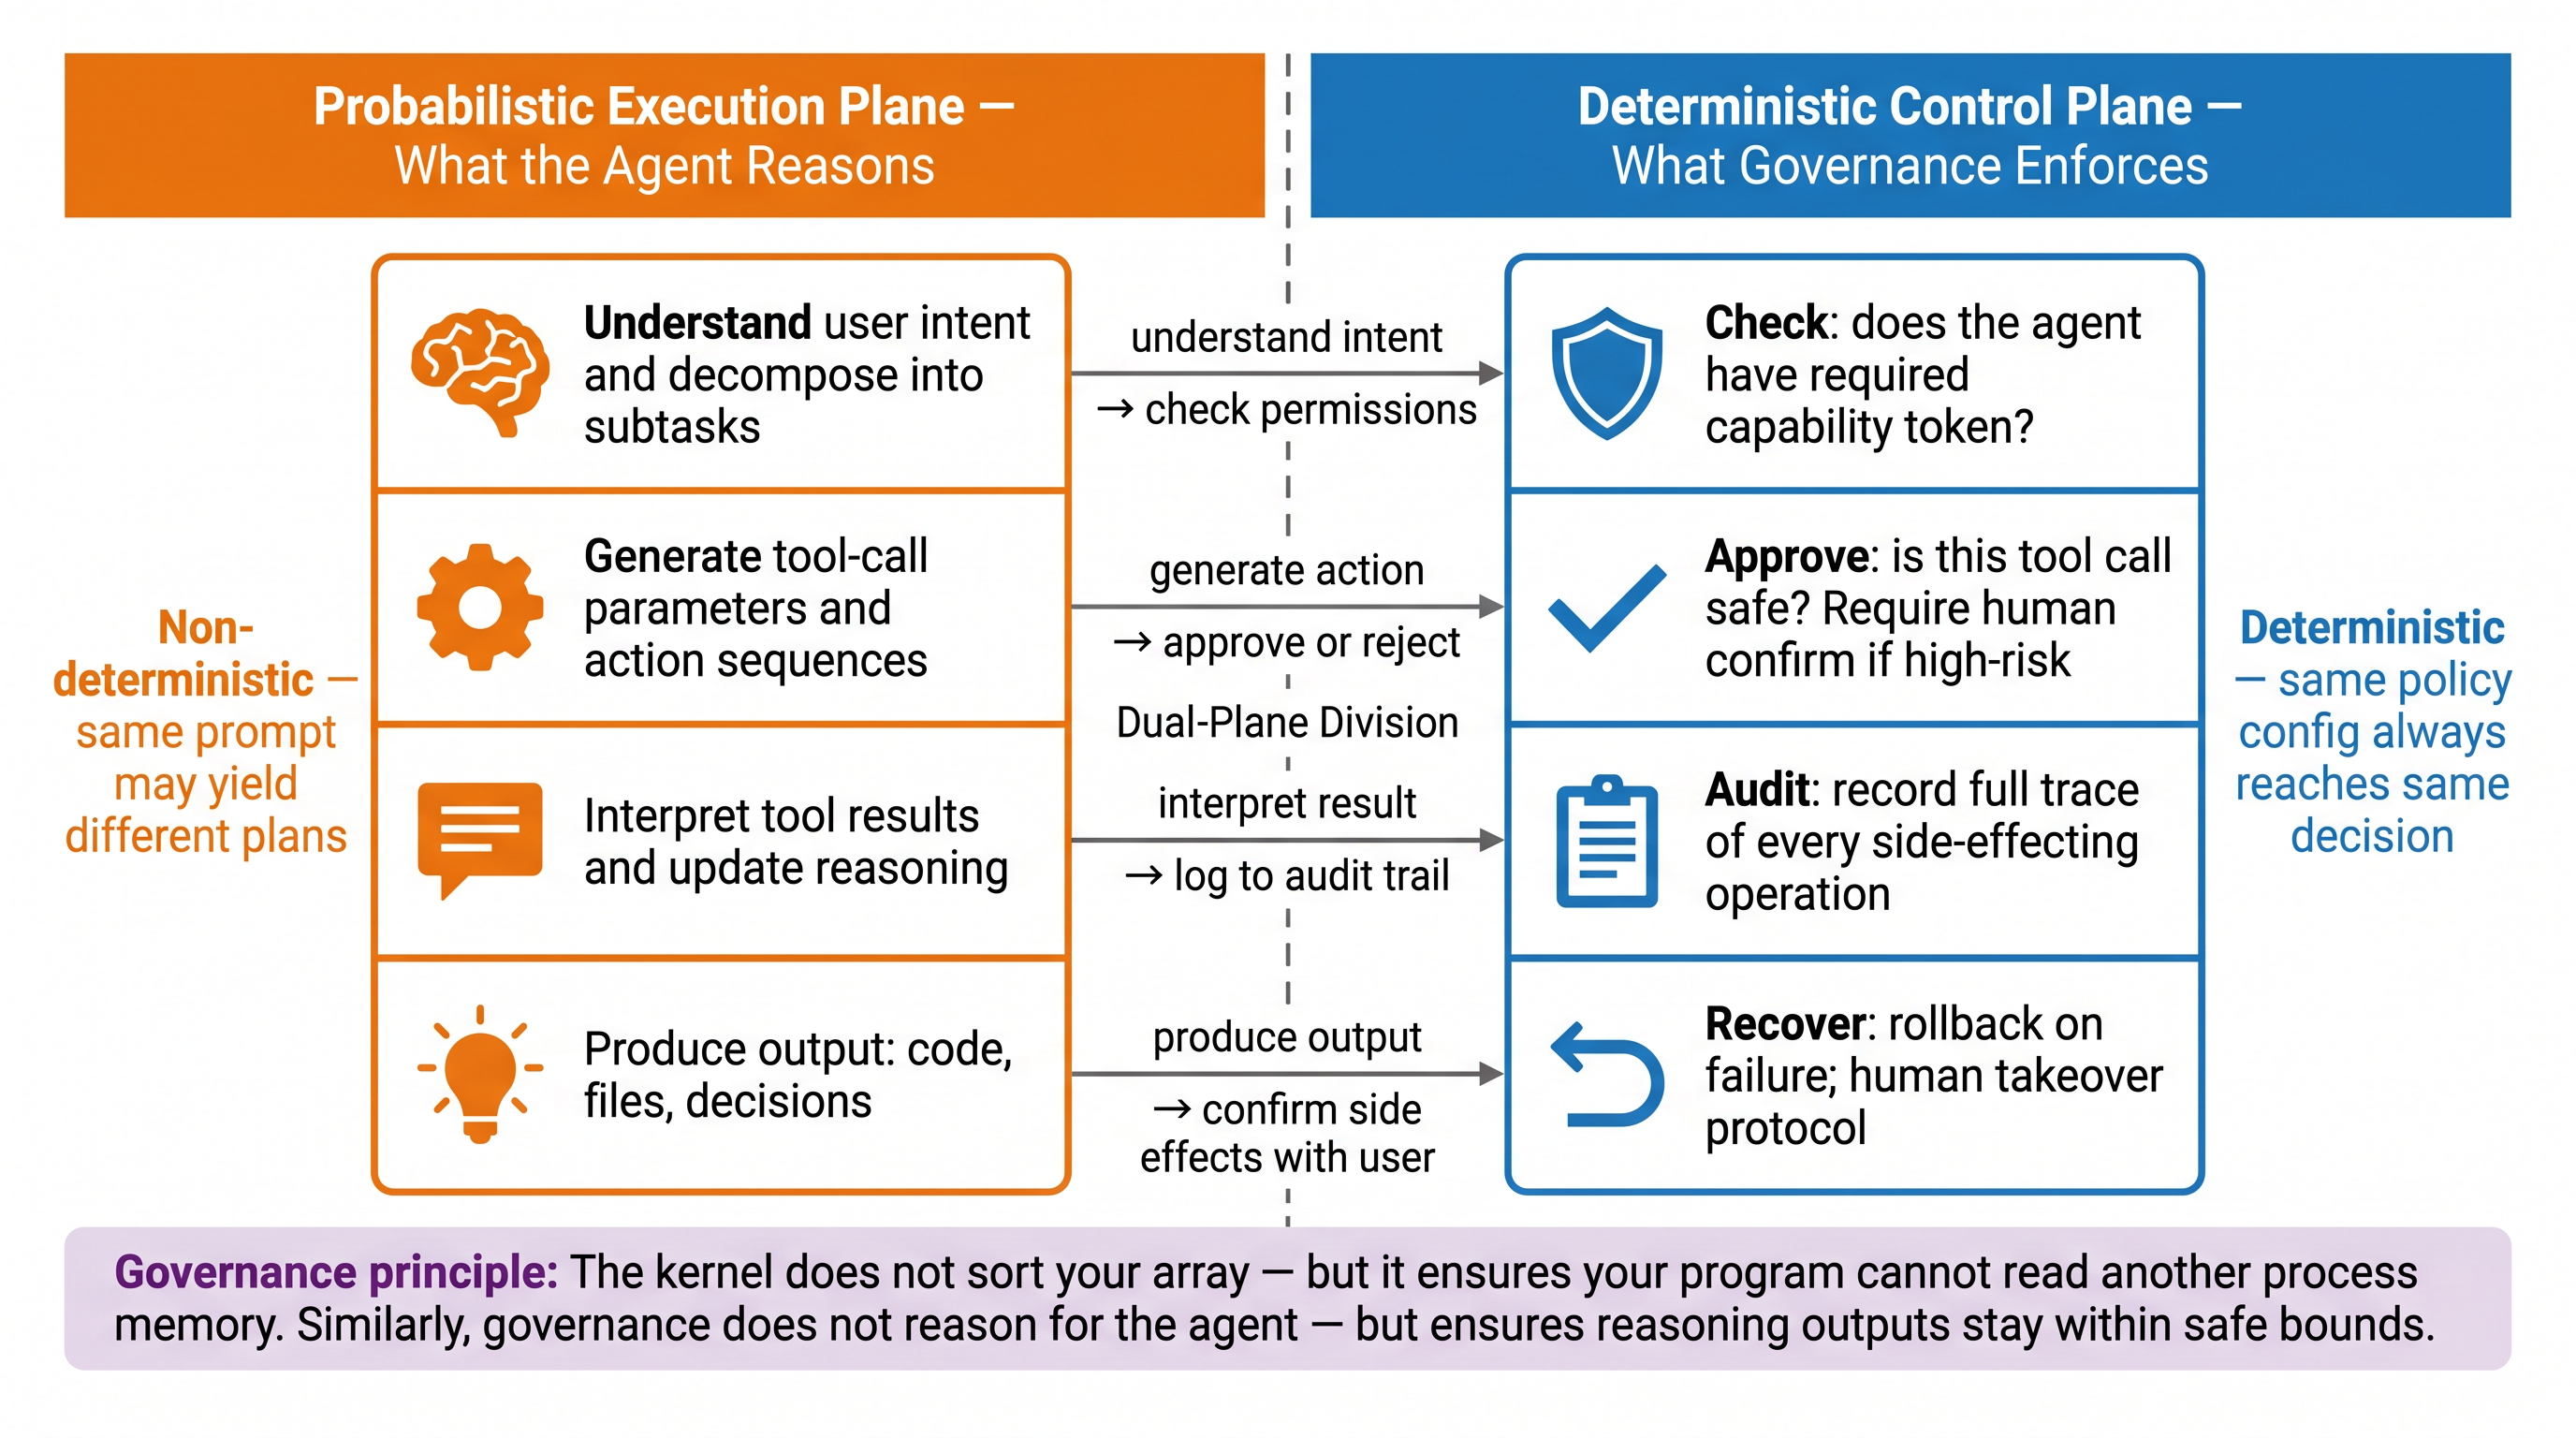
\includegraphics[width=0.90\textwidth]{figures/generated/fig_ch85_governance}
  \caption{Governance as a structural division of labor in the dual-plane architecture.
  The probabilistic execution plane (left) handles what the agent \emph{can} reason about:
  understanding user intent, generating action sequences, interpreting results, and producing outputs.
  The deterministic control plane (right) enforces what \emph{should} happen:
  checking capability permissions, approving or rejecting tool calls, maintaining a full audit trail,
  and providing rollback and human-takeover mechanisms.
  This mirrors the classical OS principle: the kernel does not sort your array,
  but it ensures your program cannot read another process's memory.
  Governance is not a retrofit layer but the structural core of the deterministic control plane,
  a first-class architectural invariant rather than an operational afterthought.}
  \label{fig:ch85:governance}
\end{figure}
